\documentclass[a4,semhelv,semrot]{seminar}
\usepackage[dvips]{graphicx}
\usepackage{fancybox}
\usepackage{a4wide}
\usepackage{amsmath}
\usepackage{amsxtra}

\newcommand{\mb}[1]{\mathbf{#1}}
\newcommand{\ket}[1]{|#1 \rangle}
\newcommand{\bra}[1]{\langle #1|}
\newcommand{\Alpha}{\bar{\alpha}}
\newcommand{\Exp}[2]{e^{i \mb{#1} \cdot \mb{#2} }}
\newcommand{\ExpM}[2]{e^{-i \mb{#1} \cdot \mb{#2} }}
\newcommand{\state}[2]{\psi_{#1 #2}}
\newcommand{\Muq}{\mu(\mb{q},\theta,\phi)}
\newcommand{\Angstrom}{\stackrel{\circ}{\mathrm{A}} }
\newcommand{\InvAngstrom}{ \stackrel{\circ}{\mathrm{A}}^{-1} } 
\newcommand{\Half}{\frac{1}{2}}

\slideframe{shadow}

\newcommand{\heading}[1]{ \begin{center}%
                          {\large {\bf \sffamily{#1}}}\\[3mm]%
                          \hrule\vspace{1mm}
                          \end{center}}
\sffamily

\begin{document}

\begin{slide}
    \heading{Bound-Bound Transition: Ground State to 1st Excited State}
    \begin{equation*}
    \eta(\mb{k},\theta,\phi) = k_x \sin\phi \cos\phi +
                               k_y \sin\phi \sin\theta +
                               k_z \cos\phi
    \end{equation*}
    \begin{equation*}
    \begin{split}
    \bra{\psi_i} \Exp{k}{r} \Alpha_j \ket{\psi_0}
    =
    \int (A_{i1}A_{01} + A_{ii}A_{0i}) R^g_{0i} \; d\Omega
    + \\
    \int (A_{i3}A_{03} + A_{i4}A_{04}) R^h_{0i} \; d\Omega
    \end{split}
    \end{equation*}

\begin{equation*}
    \mathcal{J}[a,n] = \int_0^\infty e^{-ar} r^n \; dr = \frac{\Gamma(n+1)}{a^{n+1}}
\end{equation*}
\begin{equation*}
    \mathcal{K}[a,n,A,B,C,D] = \int_0^\infty 
                \left( \frac{A-Br}{C-Dr} \right) e^{-ar} r^{n} \; dr
\end{equation*}
\end{slide}

\begin{slide}
\begin{equation*}
R^g_{01} = G_0 G'_1 \mathcal{J}[\Half(\sigma_1 + \sigma_2) - i\eta,2\gamma_1] -
           G_0 G''_1 \mathcal{J}[\Half(\sigma_1 + \sigma_2) - i\eta,2\gamma_1 + 1]
\end{equation*}

\begin{equation*}
\begin{split}
R^h_{01} = H_0 G_0 H_1 
            G'_1 \mathcal{K}[\Half(\sigma_1 + \sigma_2) - i\eta, 2\gamma_1,H'_1,H''_1,H'''_1,H''''_1]
            \\ -
   H_0 G_0 H_1          G''_1 \mathcal{K}[\Half(\sigma_1 + \sigma_2) - i\eta, 2\gamma_1,  1H'_1,H''_1,H'''_1,H''''_1]
\end{split}
\end{equation*}

\end{slide}

\begin{slide}
    \heading{The Ground State}
     \[
	\ket{1S_{\frac{1}{2}}} = \ket{0} = 
		\left(
			\begin{array}{c}
				A_{01}(\theta,\phi) \; g_0(r) \\
				A_{02}(\theta,\phi) \; g_0(r) \\
				A_{03}(\theta,\phi) \; h_0(r) \\
				A_{04}(\theta,\phi) \; h_0(r)
			\end{array}
		\right)
		=
		\left(
			\begin{array}{c}
				Y_{00} 	g_0(r)	\\
				0	 			\\
				-i \sqrt{\frac{1}{3}} Y_{10} h_0(r) \\
				-i \sqrt{\frac{2}{3}} Y_{11} h_0(r)
			\end{array}
		\right)
    \]
    %======================================================================
    \[
    \begin{array}{cc}
		g_0(r) = G_0 e^{-\frac{1}{2} \sigma_1 r} r^{\gamma_1 - 1} &
		h_0(r) = H_0 g_0(r) 
    \\
    \\
	    H_0  =  - \sqrt{ \frac{1 - \epsilon_1}{1 + \epsilon_1} }	&
	    G_0  =  \left( \frac{2Z}{a_0} \right)^{3/2} 
		  	   	\sqrt{\frac{1 + \epsilon_1}{2 \Gamma(2\gamma_1 + 1) }}
    \end{array}
    \]
\end{slide}

\begin{slide}
\heading{The First Excited State}
  \begin{equation}
	\ket{2S_{1/2}} = \ket{1} = 
		\left(
			\begin{array}{c}
				A_{11}(\theta,\phi) g_1(r) \\
				A_{12}(\theta,\phi) g_1(r) \\
				A_{13}(\theta,\phi) h_1(r) \\
				A_{14}(\theta,\phi) h_1(r)
			\end{array}
		\right)
		=
		\left(
			\begin{array}{c}
				Y_{00} 	g_1(r)	\\
				0	 			\\
				-i \sqrt{\frac{1}{3}} Y_{10} h_1(r) \\
				-i \sqrt{\frac{2}{3}} Y_{11} h_1(r)
			\end{array}
		\right)
\end{equation}
\begin{equation}
\begin{array}{cc}
	g_1(r) = e^{-\frac{1}{2} \sigma_2 r} r^{\gamma_1} 
	  		  \left( G'_{1}  \frac{1}{r} - G''_{1} \right) 
    &
   	h_1(r) = H_1 \left( \frac{H'_1 - H''_1 r}{H'''_1 - H''''_1 r} \right) g_1(r)
\end{array}
\end{equation}

\begin{equation*}
\begin{array}{cc}
	G_1 	 =  \left( \frac{2Z}{N_2 a_0} \right)^{3/2}
		  	  		\sqrt{\frac{2\gamma_1 + 1}{\Gamma(2\gamma_1 + 1)}} 
		  	  		\sqrt{\frac{1 + \epsilon_2}{4N_2 (N_2 + 1)}} 
    \; ; &
	G'_1 	 =  N_2 G_1 \sigma_2^{\gamma_1 - 1} \\
	G''_1 	 =  \left( \frac{N_2 + 1}{2\gamma_1 + 1} \right) G_1 \sigma_2^{\gamma_1}
\end{array}
\end{equation*}
\begin{equation*}
\begin{split}
\begin{array}{ccc}
	H_1 	 =  -\sqrt{\frac{1 - \epsilon_2}{1 + \epsilon_2}}  
    \; ; &
	H'_1 	 =  (2\gamma_1 + 1)(N_2 + 2)  
    \; ; &
	H''_1 	 =  (N_2 + 1)\sigma_2  
\end{array}
\\
\begin{array}{cc}
	H'''_1 	 =  (2\gamma_1 + 1)N_2  
    \; ; &
	H''''_1  =  (N_2 + 1)\sigma_2 
\end{array}
\end{split}
\end{equation*}

\end{slide}

\begin{slide}
\heading{Constants and Definitions}
    \begin{equation}
    \begin{array}{cc}
        \gamma_1 = \sqrt{1 - (\alpha Z)^2} &  \gamma_2 = \sqrt{4 - (\alpha Z)^2}
    \end{array}
\end{equation}
\begin{equation}
    \begin{array}{cccc}
        N_1 = 1 ;& N_2 = \sqrt{2(1 + \gamma_1)} ;& N_3 = 2
        ;&
        \sigma_1 = \left( \frac{2Z}{N_1 a_0} \right)
    \end{array}
\end{equation}
\begin{equation}
    \begin{array}{cc}
        \epsilon_1 = 
            \left[ 
                1 + \left( \frac{\alpha Z}{\gamma_1} \right)^2
            \right]^{-1/2}
        &
        \epsilon_2 =
            \left[ 
                1 + \left( \frac{\alpha Z}{1+\gamma_1} \right)^2
            \right]^{-1/2}
            \\
        \epsilon_3 = 
            \left[ 
                1 + \left( \frac{\alpha Z}{\gamma_2} \right)^2
            \right]^{-1/2}
    \end{array}
\end{equation}
\end{slide}

\begin{slide}
\heading{Angular Results for $f''$ at 100 eV}
\begin{center}
    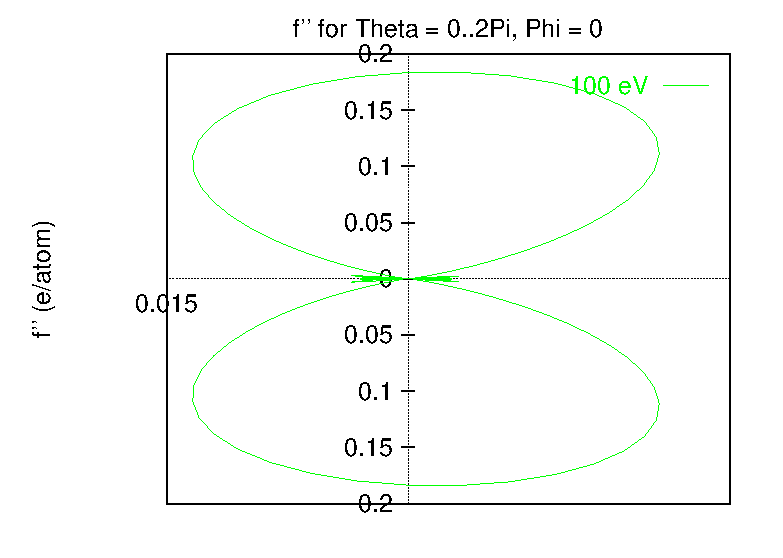
\includegraphics[width=9cm]{ANG_100.eps}
\end{center}
\end{slide}

\begin{slide}
\heading{Angular Results for $f''$ at 500 eV}
\begin{center}
    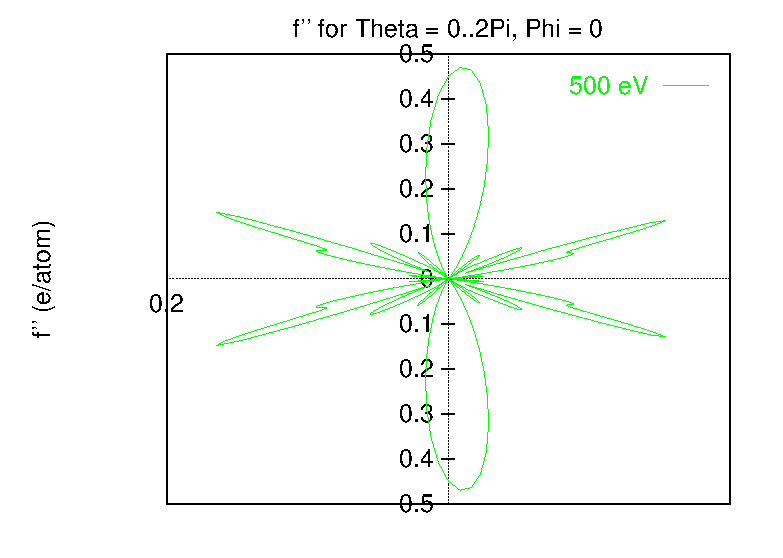
\includegraphics[width=9cm]{ANG_500.eps}
\end{center}
\end{slide}

\begin{slide}
\heading{Angular Results for $f''$ at 500 eV : E1 and AP}
\begin{center}
    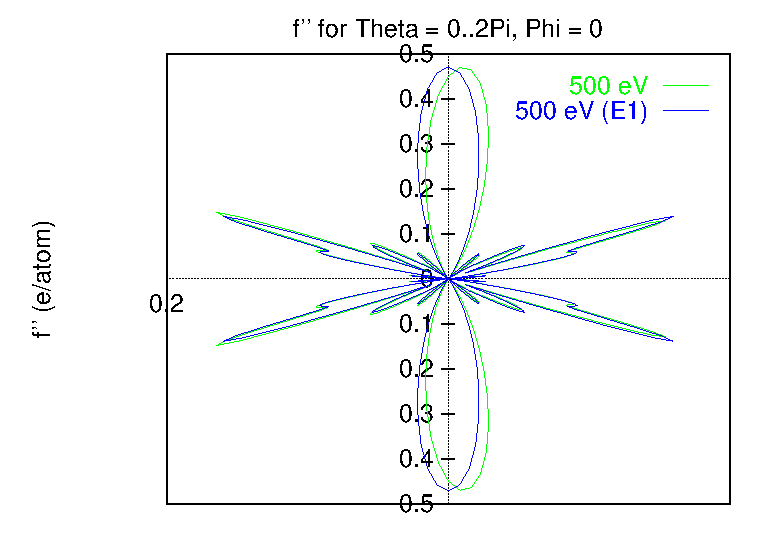
\includegraphics[width=9cm]{ANG_COMP.eps}
\end{center}
\end{slide}


\end{document}



